% ====================================================================
% VİZE RAPOR ŞABLONU – Türk Masalları Derlemesi Web Sayfası
% --------------------------------------------------------------------
% DERLEME: Overleaf'te Menu > Compiler > XeLaTeX (pdfLaTeX de çalışır).
%
% KURALLAR (şablonu kullanmadan önce okuyun):
%  1. Bölüm başlıklarını SİLMEYİN ve sırasını DEĞİŞTİRMEYİN.
%  2. [KÖŞELİ PARANTEZ] içindeki ve gri renkli açıklama metinlerini
%     kendi bilgilerinizle değiştirin; açıklama metinlerini silin.
%  3. MEBİS'e YALNIZCA bu raporun PDF'ini yükleyin.
%     ZIP ve HTML dosyası YÜKLEMEYİN. Tüm kontroller GitHub'dan yapılır.
%  4. Kapaktaki GitHub ve YouTube bağlantıları doğru ve tıklanabilir
%     olmalıdır. Teslimden önce PDF'teki bağlantılara tıklayıp deneyin.
%  5. Haftalık katkı tablosundaki görseller için resim dosyalarını
%     (hafta1.png, hafta2.png, ...) Overleaf projesine yükleyin.
%     Dosya adlarında boşluk ve Türkçe karakter kullanmayın.
%     Resim yoksa tabloda "görsel ekleyin" kutusu görünür.
%  6. Yapay zekâ kullandıysanız Bölüm 5'i doldurun.
% ====================================================================
\documentclass[12pt,a4paper]{article}

\usepackage{iftex}
\ifPDFTeX
  \usepackage[T1]{fontenc}
  \usepackage[utf8]{inputenc}
\else
  \usepackage{fontspec}
\fi
\usepackage[turkish]{babel}
\usepackage[margin=2.4cm]{geometry}
\usepackage{setspace}

\usepackage{booktabs}
\usepackage{longtable}
\usepackage{array}
\usepackage{graphicx}
\usepackage{colortbl}
\usepackage{xcolor}
\usepackage{enumitem}
\usepackage{listings}
\usepackage{amssymb}
\usepackage{caption}
\usepackage{fancyhdr}
\usepackage{hyperref}

\onehalfspacing
\setlength{\parindent}{0pt}
\setlength{\parskip}{6pt}
\setlist{itemsep=2pt, topsep=4pt}
\hypersetup{colorlinks=true, linkcolor=blue!50!black, urlcolor=blue!50!black}

\definecolor{ana}{HTML}{14325C}
\definecolor{acik}{HTML}{EEF2F8}

\lstset{basicstyle=\ttfamily\small, backgroundcolor=\color{acik},
  frame=single, rulecolor=\color{ana}, breaklines=true,
  columns=fullflexible, keepspaces=true, showstringspaces=false}

\pagestyle{fancy}
\fancyhf{}
\fancyhead[L]{\projeadi}
\fancyhead[R]{Vize Raporu}
\fancyfoot[C]{\thepage}

% ---------- Yardımcı komutlar ----------
% Gri açıklama metni (silinecek yönergeler için)
\newcommand{\aciklama}[1]{{\color{gray}\itshape (#1)}}

% Haftalık tablo görseli: dosya yoksa "görsel ekleyin" kutusu çıkar
\newcommand{\haftagorsel}[1]{%
  \IfFileExists{#1}{%
    \includegraphics[width=\linewidth,height=4.2cm,keepaspectratio]{#1}%
  }{%
    \fbox{\parbox[c][2.6cm][c]{\dimexpr\linewidth-2\fboxsep-2\fboxrule\relax}{%
      \centering\small\color{gray} Ekran görüntüsü / görsel ekleyin\\ \texttt{#1}}}%
  }%
}
% Haftalık katılım kutuları (işaretlemek için $\square$ yerine $\boxtimes$ yazın)
\newcommand{\katilimkutulari}{\par\vspace{3pt}\small $\square$ Ders içinde katılım sergiledim\par $\square$ Telafi yaptım}

% Ek görsel: dosya yoksa hiçbir şey göstermez
\newcommand{\haftaek}[1]{%
  \IfFileExists{#1}{\\[4pt]\includegraphics[width=\linewidth,height=4.2cm,keepaspectratio]{#1}}{}%
}

% ---------- Kapak bilgileri ----------
\newcommand{\universite}{İstanbul Medipol Üniversitesi / Görsel İletişim Tasarımı}
\newcommand{\dersadi}{Programlamaya Giriş}
\newcommand{\hocaadi}{Meral Şentürk}
\newcommand{\ogrenciadi}{Ceren Naz Şimşek}
\newcommand{\ogrencino}{86250002}
\newcommand{\projeadi}{Türk Masalları Derlemesi}
% Bağlantıları tam adres olarak yazın (https:// ile başlayarak)
\newcommand{\githublink}{\url{https://github.com/cerennazsimsek6/Programlama-Giri-Vize}}
\newcommand{\youtubelink}{\url{https://www.youtube.com/watch?v=E6r17uMKqPs}}

\begin{document}

% ====================================================================
% KAPAK
% ====================================================================
\begin{titlepage}
\centering
\vspace*{1cm}
{\large \universite \par}
\vspace{1.8cm}
{\Huge\bfseries\color{ana} \projeadi \par}
\vspace{0.4cm}
{\Large Türk Masalları Derlemesi Web Sayfası \par}
{\large Vize Raporu \par}
\vspace{1.8cm}
{\large \textbf{Ders:} \dersadi \par}
{\large \textbf{Öğretim Üyesi:} \hocaadi \par}
\vspace{1.2cm}
{\large \textbf{Hazırlayan:} \ogrenciadi \par}
{\large \textbf{Öğrenci No:} \ogrencino \par}
\vspace{1.8cm}
\fbox{\parbox{0.88\linewidth}{\centering\vspace{6pt}
{\large\bfseries Proje Bağlantıları}\\[8pt]
\textbf{GitHub deposu:}\\ \githublink \\[8pt]
\textbf{YouTube sunum videosu:}\\ \youtubelink
\vspace{6pt}}}
\vfill
{\large \today \par}
\end{titlepage}

\tableofcontents
\newpage

% ====================================================================
\section{Giriş}
% ====================================================================


\subsection{Proje Özeti}

Bu proje, Türk kültürünün önemli unsurlarından biri olan masalları dijital ortamda bir araya getirmek amacıyla hazırlanmıştır. Web sitesinde farklı Türk masallarına yer verilerek kullanıcıların masalları kolay ve düzenli bir şekilde incelemesi hedeflenmiştir. Proje, tek bir HTML dosyası içerisinde HTML, CSS ve JavaScript kullanılarak geliştirilmiştir. Tasarım sürecinde Türk masallarının kültürel ve geleneksel atmosferini yansıtan renkler ve görseller tercih edilmiştir. Kullanıcıların masal adlarını veya masallarla ilgili kelimeleri arayabilmesi için JavaScript ile çalışan bir arama özelliği eklenmiştir. Böylece proje, hem görsel hem de işlevsel açıdan kullanıcıların masalları kolayca keşfedebileceği bir web sayfası olarak tasarlanmıştır.

\subsection{Gereksinimlerin Karşılanması}
\begin{center}
\rowcolors{2}{acik}{white}
\begin{tabular}{@{}p{8.2cm}c@{}}
\toprule
\rowcolor{ana}\textcolor{white}{\textbf{Gereksinim}} & \textcolor{white}{\textbf{Durum}} \\
\midrule
Masal sayısı 8--12 arasında (10 masal)         & $\boxtimes$ \\
Tek HTML dosyası                                    & $\boxtimes$ \\
Stil kodları içsel (\texttt{<style>} içinde)        & $\boxtimes$ \\
Betik kodları içsel (\texttt{<script>} içinde)      & $\boxtimes$ \\
İnternetsiz açılıp çalışıyor                        & $\boxtimes$ \\
JavaScript sayfada anlamlı bir işlev görüyor        & $\boxtimes$ \\
Masal metinleri kendi cümlelerimle yazıldı          & $\boxtimes$ \\
Sayfa telefonda da düzgün görünüyor                 & $\boxtimes$ \\
\bottomrule
\end{tabular}
\end{center}


% ====================================================================
\section{Masalların Seçimi}
% ====================================================================


\begin{longtable}{@{}cp{4cm}p{3cm}p{5.4cm}@{}}
\toprule
\textbf{No} & \textbf{Masal} & \textbf{Tür} & \textbf{Seçilme nedeni} \\
\midrule
\endhead
1 & Balıkçının Oğlu & Olağanüstü masal & Geleneksel Türk masallarındaki macera ve mücadele unsurlarını yansıttığı için seçildi. \\
2 & Bıyık Balta ve Şehzade & Olağanüstü masal & Fantastik karakterleri ve macera dolu anlatımı nedeniyle seçildi. \\
3 & Değirmenci ile Tilki & Hayvanlı masal & Tilki karakteri üzerinden zekâ ve kurnazlık temasını yansıttığı için seçildi. \\
4 & Fatmacık ile Yusufçuk & Olağanüstü masal & Halk anlatılarındaki sevgi, dostluk ve mücadele temalarını içerdiği için seçildi. \\
5 & İncili Çadır & Olağanüstü masal & Gizemli ve fantastik olaylara yer vermesi nedeniyle seçildi. \\
6 & Kırk Dost Masalı & Olağanüstü masal & Dostluk ve dayanışma temasını geleneksel bir anlatımla ele aldığı için seçildi. \\
7 & Korkak Adam ve Devler & Dev masalı & Devler ve olağanüstü olaylar içeren fantastik yapısı nedeniyle seçildi. \\
8 & Leylek Dadı ile Fakir Köylü Kızı & Olağanüstü masal & Farklı karakterleri ve geleneksel masal öğelerini bir araya getirdiği için seçildi. \\
9 & Mitişik Kız & Olağanüstü masal & Geleneksel anlatı özellikleri ve fantastik olay örgüsü nedeniyle seçildi. \\
10 & Derviş & Halk masalı & Geleneksel kültürel ve manevi unsurları yansıttığı için seçildi. \\
\bottomrule
\end{longtable}

% ====================================================================
\section{Tasarım Kararları}
% ====================================================================


\subsection{Konuya Uygunluk}
Web sitesinin tasarımında Türk masallarının kültürel ve geleneksel atmosferini yansıtan bir görsel dil oluşturulmuştur. Tasarımda sıcak ve doğal renk tonları kullanılarak masalların geleneksel yapısıyla uyum sağlanması amaçlanmıştır. Masal kartlarında kullanılan görseller, kullanıcıların her masalı daha kolay tanımasına ve içerikle görsel bir bağ kurmasına yardımcı olmaktadır. Sayfa düzeninde sade ve anlaşılır bir yapı tercih edilerek kullanıcıların masallar arasında rahatça gezebilmesi hedeflenmiştir. Böylece tasarım kararları, hem Türk masalları temasını desteklemiş hem de kullanıcı deneyimini güçlendirmiştir.

\subsection{Renk Paleti ve Yazı Tipi}
\begin{center}
\rowcolors{2}{acik}{white}
\begin{tabular}{@{}llp{6.4cm}@{}}
\toprule
\rowcolor{ana}\textcolor{white}{\textbf{Ad}} & \textcolor{white}{\textbf{Kod}} & \textcolor{white}{\textbf{Nerede / neden kullandınız?}} \\
\midrule
Koyu mor & \texttt{\#65416D} & Butonlar ve vurgu alanlarında kullanıldı. Masalsı ve sıcak bir görünüm sağlıyor. \\
Koyu lacivert-mor & \texttt{\#392E43} & Alt bilgi bölümünde kullanıldı ve tasarıma güçlü bir kontrast kattı. \\
Açık krem & \texttt{\#FFF4E6} & Açık alanlarda kullanılarak sıcak ve rahat bir okuma ortamı oluşturuldu. \\
Açık yeşil & \texttt{\#E8EFE5} & Bilgilendirme alanlarında kullanıldı. Doğal atmosferi destekliyor. \\
Sistem yazı tipi & Arial, sans-serif & İnternetsiz çalışmayı sağlamak ve okunabilirliği korumak için tercih edildi. \\
\bottomrule
\end{tabular}
\end{center}

\subsection{Okunabilirlik, Gezinme ve Duyarlı Tasarım}
\begin{itemize}
  \item \textbf{Okunabilirlik:} Açık krem arka plan üzerinde koyu renkli metinler kullanılarak yazıların kolay okunması sağlandı.
\item \textbf{Gezinme:} Kullanıcılar arama kutusu ve kategori butonları sayesinde istedikleri masala kolayca ulaşabilmektedir.
\item \textbf{Duyarlı tasarım:} Sayfa, farklı ekran boyutlarında düzenli görünecek şekilde esnek bir yapı ile tasarlandı.
\item \textbf{Tutarlılık:} Başlıklar, renkler, butonlar ve masal kartlarında aynı görsel dil kullanılarak bütünlük sağlandı.
\end{itemize}

\subsection{Ekran Görüntüleri}


\begin{figure}[h]
  \centering
\resizebox{0.65\textwidth}{!}{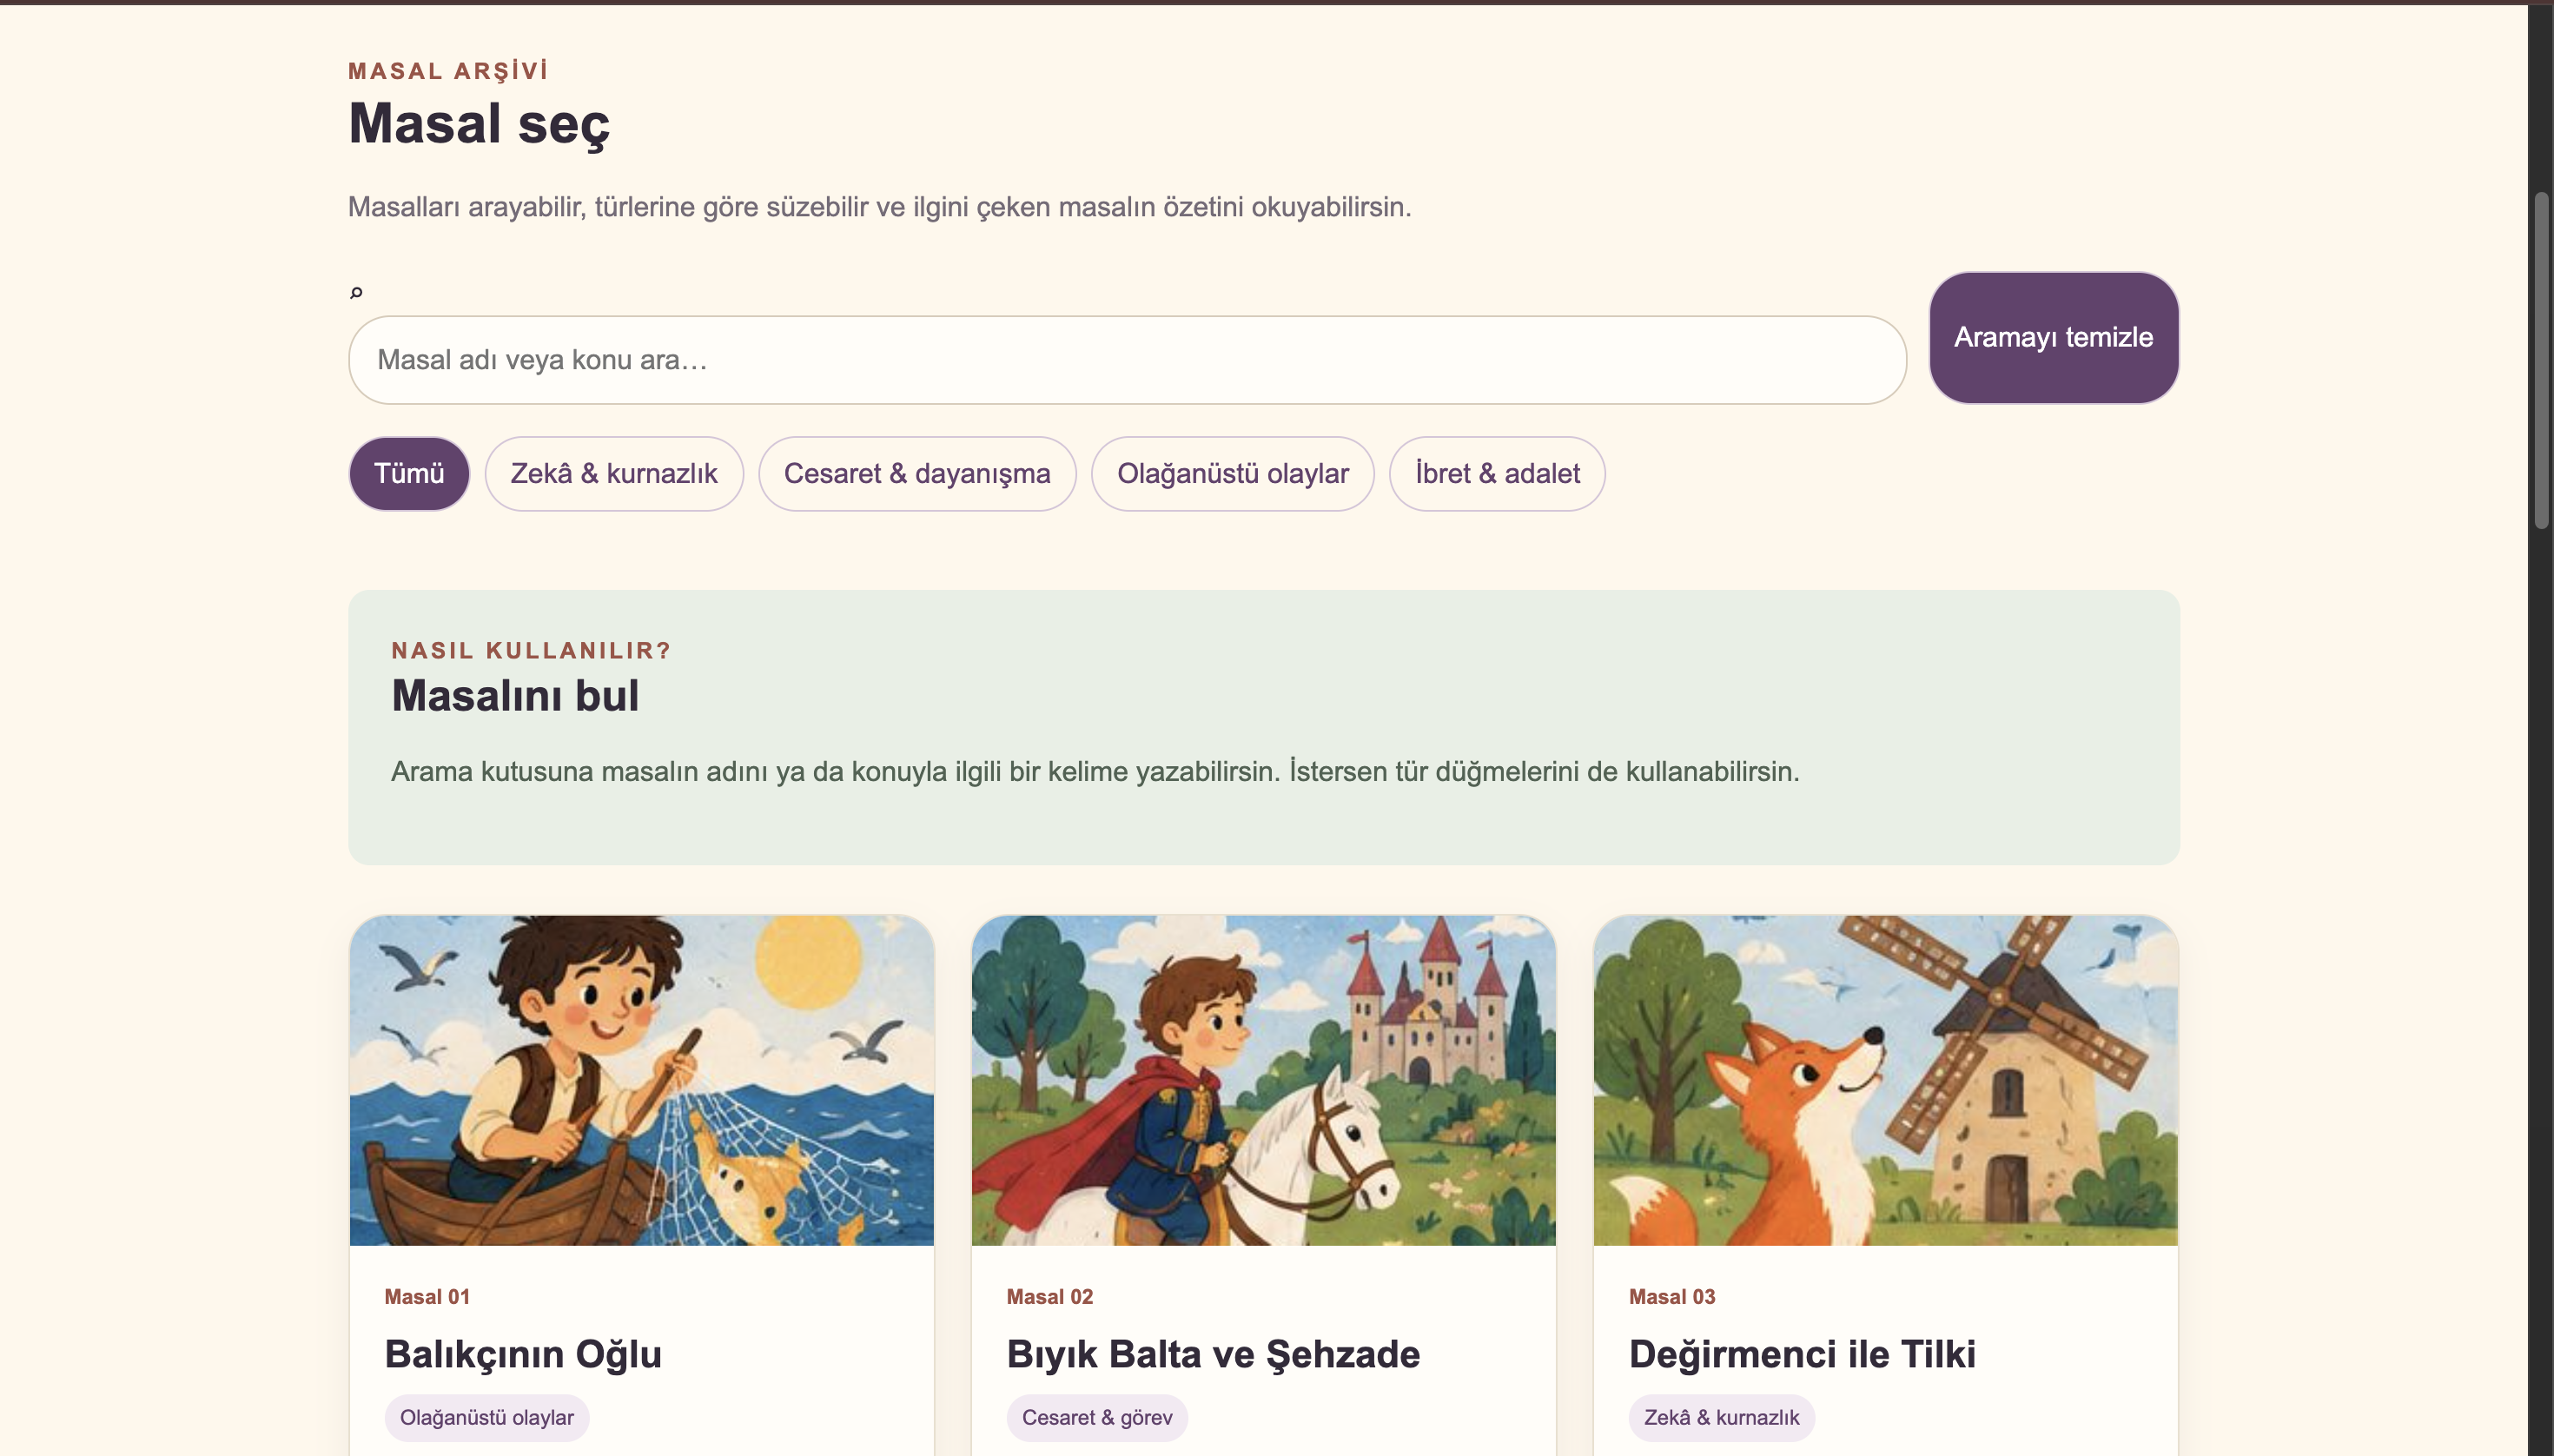
\includegraphics{foto1.png}}
  \caption{Sayfanın bilgisayar görünümü}
 \end{figure}
\begin{figure}
  \centering
\resizebox{0.20\textwidth}{!}{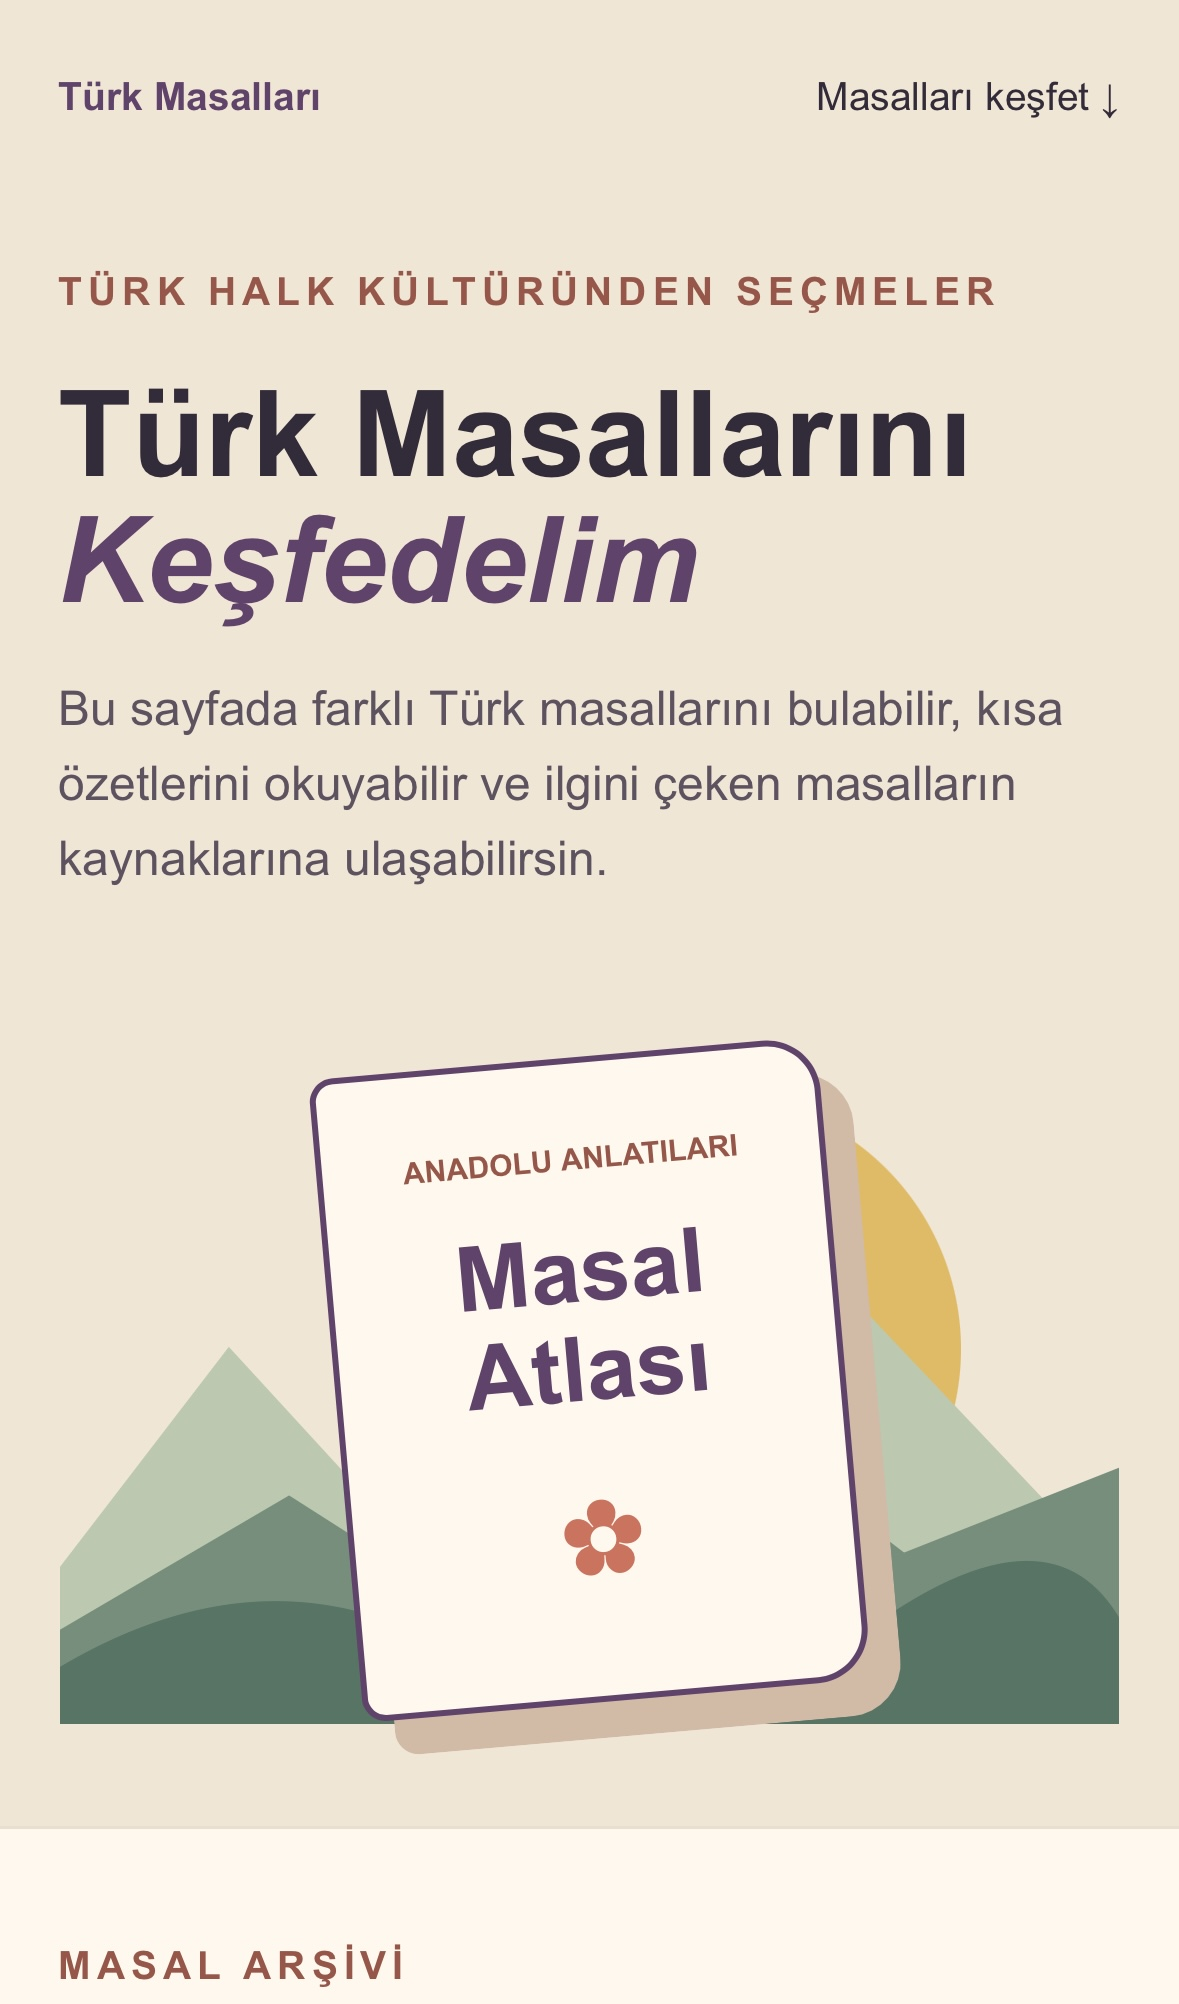
\includegraphics{foto2.jpg}}
   \caption{Sayfanın telefon görünümü}
\end{figure}

% ====================================================================
\section{Gerçekleştirme}
% ====================================================================


\subsection{HTML Yapısı}
Web sitesi tek bir HTML dosyası içerisinde oluşturulmuştur. Sayfada üst menü, tanıtım alanı, masal arşivi, arama bölümü ve masal kartları gibi temel bölümler bulunmaktadır. HTML etiketleri kullanılarak sayfanın yapısı düzenli ve anlaşılır bir şekilde oluşturulmuştur.

\subsection{İçsel CSS}
Web sitesinin görsel tasarımı için CSS kodları HTML dosyasının içerisinde kullanılmıştır. Renkler, yazı tipleri, boşluklar, butonlar ve masal kartlarının düzeni CSS ile belirlenmiştir. Ayrıca farklı ekran boyutlarında düzenli bir görünüm sağlamak amacıyla duyarlı tasarım kurallarından yararlanılmıştır.

\begin{lstlisting}[caption={İçsel CSS'ten önemli bir bölüm}]
.story-card {
    border-radius: 12px;
    padding: 15px;
}
\end{lstlisting}

\subsection{İçsel JavaScript}
Web sitesinde JavaScript kullanılarak kullanıcı etkileşimi sağlanmıştır. Arama kutusuna girilen kelimelere göre masallar filtrelenebilmekte ve kategori butonları kullanılarak masallar türlerine göre görüntülenebilmektedir. Ayrıca kullanıcıların sayfa içerisinde daha kolay gezinebilmesi için etkileşimli işlevlerden yararlanılmıştır.

\begin{lstlisting}[caption={İçsel JavaScript'ten önemli bir bölüm}]
const searchInput = document.getElementById("searchInput");

searchInput.addEventListener("input", function() {
    filterStories();
});
\end{lstlisting}

\subsection{Sayfanın Özellikleri}


% ====================================================================
\section{Yapay Zekâ Kullanımı}
% ====================================================================


\begin{longtable}{@{}p{2.6cm}p{3.6cm}p{4.2cm}p{3.4cm}@{}}
\toprule
ChatGPT & Kod geliştirme ve açıklama & Web sayfasının kod yapısı ve rapor metinleri için destek alındı & Kod ve rapor bölümleri \\
\midrule

ChatGBT & Görsel üretimi & Masallarda kullanılan özgün illüstrasyonların oluşturulması & Masal kartları \\
\bottomrule
\end{longtable}

\subsection{Anladığım ve Kendim Yaptığım Kısımlar}

Web sayfasının HTML yapısını oluştururken başlık, arama alanı, kategori butonları ve masal kartlarının nasıl düzenlendiğini öğrendim. CSS kullanarak sayfanın renklerini, yazı tiplerini ve yerleşimini düzenledim. JavaScript bölümünde ise arama ve kategori filtreleme özelliklerinin çalışma mantığını inceleyerek kodları kendi projemde uyguladım. Yapay zekâdan aldığım önerileri projenin gereksinimlerine göre düzenleyip test ederek kullandım.

% ====================================================================
\section{Haftalık Katkılar}
% ====================================================================


\begin{longtable}{@{}>{\raggedright\arraybackslash}p{1.7cm}
                    >{\raggedright\arraybackslash}p{6.5cm}
                    >{\centering\arraybackslash}p{6cm}@{}}

\rowcolor{ana}\textcolor{white}{\textbf{Hafta}} &
\textcolor{white}{\textbf{Yapılan çalışma}} &
\textcolor{white}{\textbf{Görsel}} \\
\hline

\textbf{1. hafta}\newline 23 Eylül 2026 &
Bu çalışmada HTML'in temel yapısı öğrenilerek WorldWideWeb konulu bir web sayfası oluşturulmuştur. Başlık, paragraf ve bağlantı etiketleri kullanılarak sayfa içeriği düzenlenmiştir. \newline \textbf{Commit:} Henüz eklenmedi. \newline $\boxtimes$ Ders içinde katılım sergiledim
\newline $\square$ Telafi yaptım & 
\begin{minipage}[t]{\linewidth}
  \vspace{0pt}
  \centering
  \haftagorsel{hafta1.png}
\end{minipage} \\
\midrule

\textbf{2. hafta}\newline 30 Eylül 2026 &
Bu çalışmada JavaScript kullanılarak butonlara tıklama ve fare hareketleriyle çalışan basit etkileşimler oluşturulmuştur. Bağlantıların aynı ve yeni sekmede açılması ile fare üzerine gelindiğinde yazı renginin değiştirilmesi uygulamaları yapılmıştır. Ayrıca ders kapsamında bir ödev verilmiştir. \newline \textbf{Commit:} Henüz eklenmedi. \newline $\boxtimes$ Ders içinde katılım sergiledim
\newline $\square$ Telafi yaptım & 
\begin{minipage}[t]{\linewidth}
  \vspace{0pt}
  \centering
  \haftagorsel{hafta2.png}
\end{minipage} \\
\midrule

\textbf{3. hafta}\newline 7 Ekim 2026 &
Bu çalışmada JavaScript ile kullanıcı etkileşimine yönelik uygulamalar yapılmıştır. Kullanıcıdan alınan verinin kontrol edilmesi, butona tıklandığında ekrana mesaj yazdırılması ve sayıyı artırıp sıfırlayabilen basit bir sayaç uygulaması oluşturulmuştur. \newline \textbf{Commit:} Henüz eklenmedi. \newline $\boxtimes$ Ders içinde katılım sergiledim
\newline $\square$ Telafi yaptım & 
\begin{minipage}[t]{\linewidth}
  \vspace{0pt}
  \centering
  \haftagorsel{hafta3.png}
\end{minipage} \\
\midrule

\textbf{4. hafta}\newline 14 Ekim 2026 &
Bu çalışmada JavaScript ile sayfalar arası yönlendirme işlemleri ve butonlara tıklama olayları uygulanmıştır. Ayrıca kartların tıklanma durumlarını kontrol ederek eşleşen ve eşleşmeyen kartlara farklı işlemler uygulayan basit bir renk eşleştirme oyunu oluşturulmuştur. \newline \textbf{Commit:} Henüz eklenmedi. \newline $\boxtimes$ Ders içinde katılım sergiledim
\newline $\square$ Telafi yaptım & 
\begin{minipage}[t]{\linewidth}
  \vspace{0pt}
  \centering
  \haftagorsel{hafta4.png}
\end{minipage} \\
\midrule

\textbf{5. hafta}\newline 21 Ekim 2026 &
Bu çalışmada HTML, CSS ve JavaScript dosyalarının birlikte kullanımı öğrenilmiştir. Harici CSS kullanılarak web sayfasının görünümü düzenlenmiş, JavaScript ile bir butona tıklandığında kutunun arka plan rengini değiştiren basit bir etkileşim uygulaması yapılmıştır. \newline \textbf{Commit:} Henüz eklenmedi. \newline $\boxtimes$ Ders içinde katılım sergiledim
\newline $\square$ Telafi yaptım & 
\begin{minipage}[t]{\linewidth}
  \vspace{0pt}
  \centering
  \haftagorsel{hafta5.png}
\end{minipage} \\
\midrule
\end{longtable}

% ====================================================================
\section{Test ve Değerlendirme}
% ====================================================================

\begin{center}
\rowcolors{2}{acik}{white}
\begin{tabular}{@{}p{6cm}p{3.4cm}p{3.4cm}@{}}
\toprule
\rowcolor{ana}\textcolor{white}{\textbf{Özellik}} & \textcolor{white}{\textbf{Bilgisayar}} & \textcolor{white}{\textbf{Telefon}} \\
\midrule
\relax Buton & Çalışıyor  & Çalışıyor \\
\relax Arama Motoru & Çalışıyor & Çalışıyor \\
\end{tabular}
\end{center}

\textbf{Denenen tarayıcılar:} [Chrome, Firefox, Edge, Safari vb.]

% ====================================================================
\section{Sunum Videosu}
% ====================================================================
\begin{center}
\begin{tabular}{@{}ll@{}}
\textbf{Video süresi:} & 12:00 \quad \aciklama{12--18 dakika olmalıdır} \\
\textbf{Görünürlük:} & Herkese açık \\
\textbf{Bağlantı:} & \youtubelink \\
\end{tabular}
\end{center}

\subsection{Video Kontrol Listesi}
\begin{itemize}
  \item $\boxtimes$ Süre 12--18 dakika aralığında.
  \item $\boxtimes$ Sunum boyunca kameram açık, yüzüm görünüyor.
  \item $\boxtimes$ Görünürlük \textbf{Listelenmemiş} (ya da Herkese açık); \textbf{Özel} değil.
  \item $\boxtimes$ Bağlantıyı gizli pencerede açtım, video oynuyor.
  \item $\boxtimes$ YouTube videoyu işlemeyi bitirdi.
  \item $\boxtimes$ Videoyu baştan sona izledim; ses ve kamera tüm sunumda var.
  \item $\boxtimes$ Kapaktaki bağlantı ile bu bölümdeki bağlantı aynı.
\end{itemize}

% ====================================================================
\section{Sonuç ve Kendi Değerlendirmem}
% ====================================================================


Bu proje sayesinde HTML, CSS ve JavaScript'in bir web sitesinde birlikte nasıl kullanılabildiğini daha iyi öğrendim. HTML ile sayfanın temel yapısını oluştururken, CSS ile görsel düzenlemeler yaptım. JavaScript kullanarak masalların aranması ve kategorilere göre filtrelenmesi gibi etkileşimli özellikler ekledim. Proje sürecinde en çok farklı bölümleri birbiriyle uyumlu şekilde düzenlerken zorlandım. Karşılaştığım sorunları kodları tekrar kontrol ederek ve uygulamaları test ederek çözmeye çalıştım. Ayrıca web sayfasının farklı ekranlarda nasıl göründüğünü inceleyerek gerekli düzenlemeleri yaptım. İleride projeyi daha fazla etkileşimli özellik ve daha gelişmiş bir tasarımla geliştirmek isterdim.

% ====================================================================
\section{Kaynakça}

\begin{thebibliography}{9}

\bibitem{k1} T.C. Kültür ve Turizm Bakanlığı. \emph{Masallar}. e-Kitap. Erişim tarihi: 21 Ekim 2026.

\bibitem{k2} T.C. Kültür ve Turizm Bakanlığı. \emph{Masallar}. Kültür Portalı. Erişim tarihi: 21 Ekim 2026.

\bibitem{k3} Masal Sitesi. \emph{Türk Masalları ve Masal Arşivi}. Erişim tarihi: 21 Ekim 2026.

\bibitem{k4} MDN Web Docs. \emph{HTML, CSS ve JavaScript Dokümantasyonu}. Erişim tarihi: 3 Kasım 2026.

\bibitem{k5} OpenAI. (2026). \emph{ChatGPT}. Projenin kod geliştirme, içerik düzenleme ve raporlama süreçlerinde yapay zekâ desteği amacıyla kullanılmıştır.

\end{thebibliography}


% ====================================================================
\appendix
\section{Teslim Kontrol Listesi}
% ====================================================================

\begin{itemize}
  \item $\boxtimes$ MEBİS'e \textbf{yalnızca bu raporun PDF'ini} yükleyeceğim. ZIP ve HTML dosyası yüklemeyeceğim.
  \item $\boxtimes$ PDF dosya adı \texttt{OgrenciNo\_AdSoyad\_vize.pdf} biçiminde.
  \item $\boxtimes$ Kapaktaki GitHub ve YouTube bağlantıları doğru; PDF'te tıklayıp denedim.
  \item $\boxtimes$ GitHub deposunda web sayfası (tek \texttt{.html}), rapor PDF'i, \texttt{.tex} kaynakları ve \texttt{README.md} var.
  \item $\boxtimes$ GitHub deposu \textbf{herkese açık} (ya da öğretim üyesine erişim verdim).
  \item $\boxtimes$ Çalışmamın son hâli teslim saatinden \textbf{önce} depoya gönderildi (sonraki commitler değerlendirilmez).
  \item $\boxtimes$ Sayfa içsel CSS ve içsel JavaScript kullanıyor, harici dosya gerektirmiyor.
  \item $\boxtimes$ Hazır taslak kullanmadım; yapay zekâ kullandıysam Bölüm 5'i doldurdum.
  \item $\boxtimes$ Çalışmanın mantığını sunumda anlatabilirim.
\end{itemize}

\end{document}